\documentclass{article}
\usepackage[utf8]{inputenc}
\usepackage[margin=0.8in]{geometry}
\usepackage{graphicx}
\title{MoView}
\author{Himaja }
\date{September 2021}
\begin{document}
\maketitle
\flushleft
\newpage
\section{Introduction}
\vspace{10pt}
\textbf{What is IMDB?} 
\vspace{5pt}
\newline 
It is acronym for Internet Movie DataBase.It gives us information about movies,shows ratings,reviews,duration,critic reviews..
\vspace{10pt}
\newline
\textbf{Inspiration}
\vspace{5pt}
\newline
Artificial Intelligence is special tool which helps us to get the predictions efficiently.IMDB consists of databases which gives us information about both shows and movies.I am actually trying to create a tool which gives us data about only movies.
\vspace{5pt}
\newline
IMDB search engine does not gives us data when the search is based on ratings or reviews.This tool also consists a special feature which helps us to predict the rating of upcoming releases. 
\section{Data Base}
\vspace{5pt}
The data base used in this project consists of 7 attributes along with result attribute which is built based on movies with rating more than 6.3 is considered as '1' otherwise '0' condition.The seen attributes are Name of the movies,Number of review,Duration of the Movie,Number of critic reviews,Release year,Rating,Release Year.This data base is collected from website Itronix Solutions.
\vspace{10pt}
\newline
Reference link:
https://www.itronixsolutions.com/imdb-movies-data-cleaning-and-data-analysis-using-python/
\subsection{3-D Plot}
\begin{figure}
\end{figure}
\begin{center}
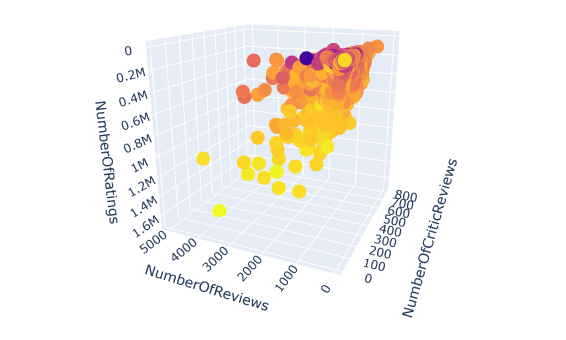
\includegraphics[scale=0.5]{3D_Plot}
\label{figure}
\end{center}
\subsection{Data Set}
\begin{figure}
\end{figure}
\begin{center}
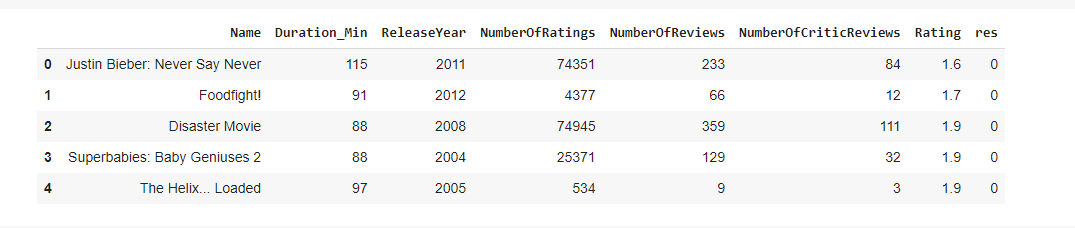
\includegraphics[scale=0.5]{DataBase}
\label{figure}
\end{center}
\newpage
\subsection{Input Statistics}
\begin{figure}
\end{figure}
\begin{center}
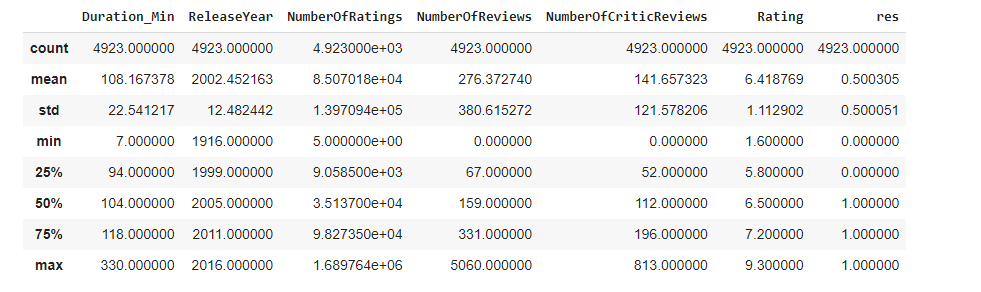
\includegraphics[scale=0.5]{Count}
\label{figure}
\end{center}
\vspace{10pt}
\begin{figure}
\end{figure}
\begin{center}
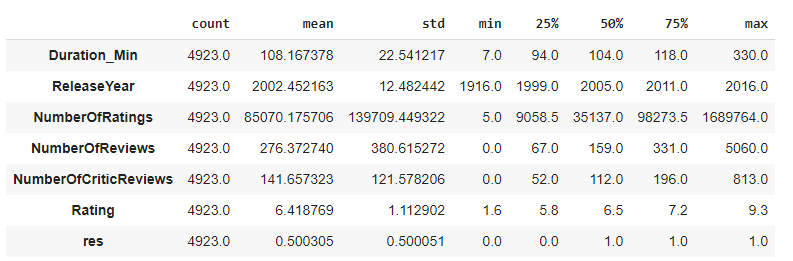
\includegraphics[scale=0.5]{Descri}
\label{figure}
\end{center}
\begin{figure}
\end{figure}
\begin{center}
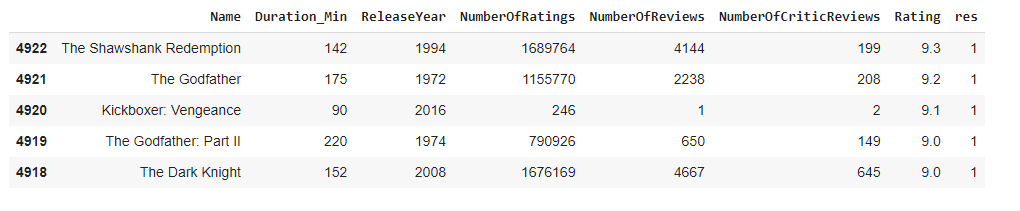
\includegraphics[scale=0.5]{Descri1}
\label{figure}
\end{center}
\section{Data Prepossessing}
Data preprocessing can refer to manipulation or dropping of data before it is used in order to ensure or enhance performance, and is an important step in the data mining process
\begin{figure}
\end{figure}
\subsection{Data Normalization}
Database normalization is the process of structuring a database, usually a relational database, in accordance with a series of so-called normal forms in order to reduce data redundancy and improve data integrity.
\begin{figure}
\end{figure}
\begin{center}
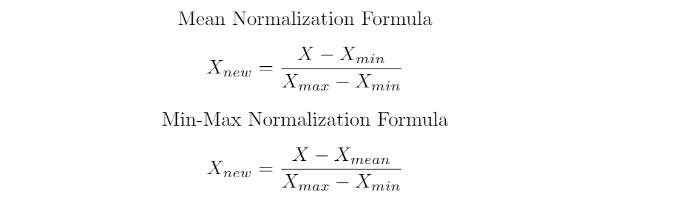
\includegraphics[scale=0.5]{Normalization.png}
\label{figure}
\end{center}
\subsection{Normalized Data}
\begin{center}
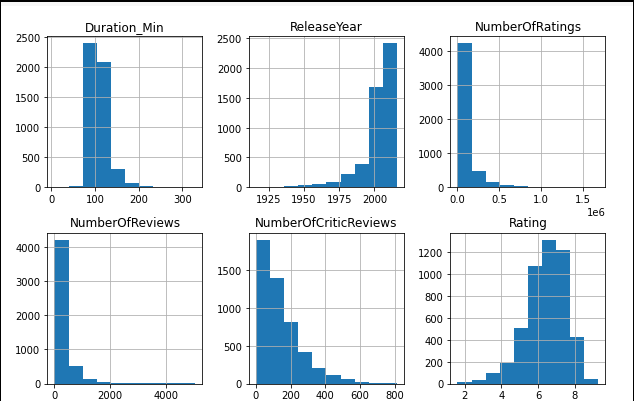
\includegraphics[scale=0.5]{Graph.png}
\label{figure}
\end{center}
\begin{figure}
\end{figure}
\begin{center}
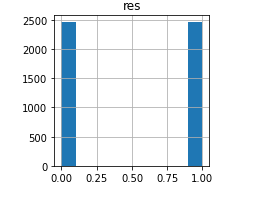
\includegraphics[scale=0.5]{Graph1}
\label{figure}
\end{center}
\subsection{Rating VS Critic Reviews}
\begin{figure}
\end{figure}
\begin{center}
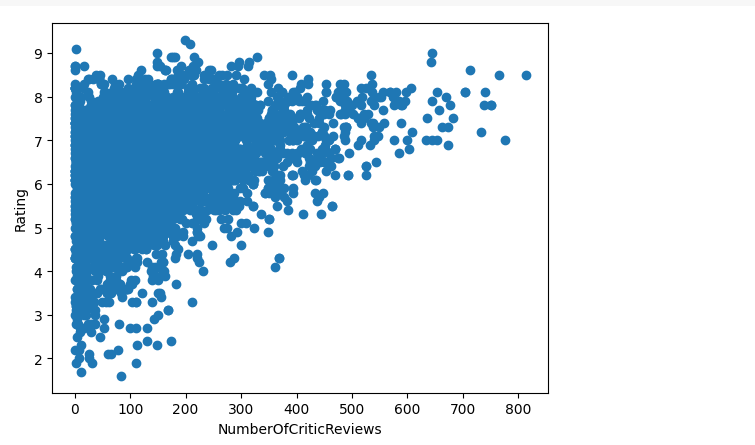
\includegraphics[scale=0.5]{Graph2}
\label{figure}
\end{center}
\subsection{Data}
\begin{figure}
\end{figure}
\begin{center}
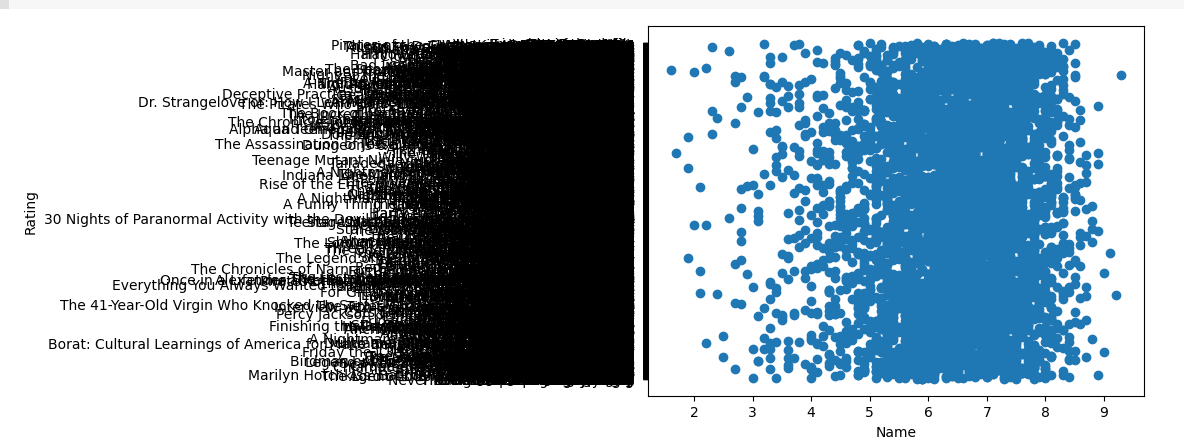
\includegraphics[scale=0.5]{Names Attribute}
\label{figure}
\end{center}
\subsection{Data}
\begin{figure}
\end{figure}
\begin{center}
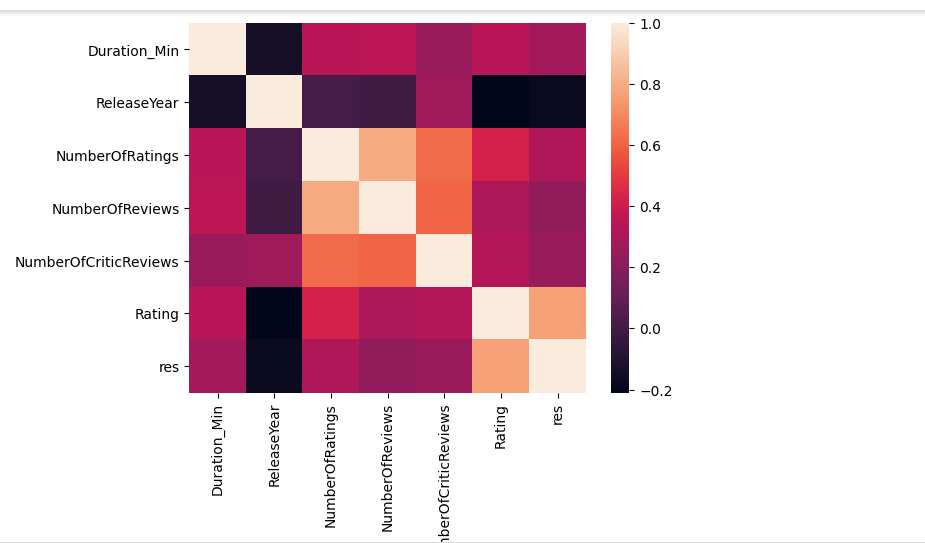
\includegraphics[scale=0.5]{Data1}
\label{figure}
\end{center}
\section{Data Analysis}
\subsection{To Be Continued...}
\section{Modelling}
\subsection{To Be Continued...}
\section{Evaluation}
\subsection{To Be Continued...}
\section{Conclusion}
\subsection{To Be Continued...}
\newpage
\bibliographystyle{unsrt}
\bibliography{report}
[1] IMDB website:  https://www.imdb.com/
\newline
[2] Intronix Solutions: https://itronixsolution.com/
\end{document}